\documentclass{article}

% ICLR 2027 official style files (downloaded from media.iclr.cc).
\usepackage{iclr2027_conference,times}

\input{math_commands.tex}

\usepackage{amsthm}
\usepackage{booktabs}
\usepackage{graphicx}
\usepackage{hyperref}
\usepackage{url}

\newtheorem{proposition}{Proposition}
\newtheorem{corollary}{Corollary}
\newcommand{\kmix}{\kappa_{\mathrm{mix}}}
\newcommand{\kep}{\kappa_{\mathrm{ep}}}
\newcommand{\gbar}{\bar{g}}

\title{Auditing Gradient Retention under Hidden Conditions:\\
Exact Cancellation, Objective-Dependent Alignment,\\
and the Limits of Kappa}

% Submission must be anonymous: do not list authors in the submitted version.
\author{Anonymous authors\\Paper under double-blind review}

\newcommand{\fix}{\marginpar{FIX}}
\newcommand{\new}{\marginpar{NEW}}

%\iclrfinalcopy % Uncomment for camera-ready version, but NOT for submission.
\begin{document}

\maketitle

\begin{abstract}
Learning systems often average gradients over hidden conditions: annotator
groups with conflicting preferences, clients with different objectives,
hidden teammates. When does averaging aggregate useful signal, and when does
it suppress it? We show that gradient cancellation is governed by more than
the presence of hidden heterogeneity. In an analytically tractable mirror
model, elementwise parameter-independent weight fields cancel exactly under a
symmetric condition mixture, while a differentiable-baseline field can retain
a nonzero component away from uniform policies. For $K$-way mixtures retention
depends on the mixture direction in the probability simplex at fixed distance
from uniform, and objective-induced channels can interfere, making retention
non-monotone in the entropy weight. A measurement protocol separates these
structural effects from finite-sample noise: deterministic rollouts collapse
retention into a weight ratio, and episode-noise readouts can understate it by
an order of magnitude. Under a single
bounded definition the retention score alone is ambiguous: a high score can
be produced by condition-blindness rather than survival. In Overcooked the
dynamic value field scores $0.998$ while its condition contrast is only
$0.1\%$ of its shared mass; the differentiable-baseline advantage field
carries a resolvable contrast ($35$--$176\times$ the estimation-noise floor,
score $0.590$) and the plain policy gradient's contrast sits at the noise
floor (score $0.529$). In 510K no field has a substantial condition
contrast. The $30$--$65\times$ value--policy gap suggested by noisy readouts
is retired. A
controlled capacity experiment shows that severe cancellation can coexist with
poor worst-condition performance; in contrast, on a real three-group
preference dataset the condition-contrast energy is dominated by item-level
noise and group-conditioned capacity yields no gain. In a switching task,
retention need not predict return when the measured condition is not the
variable the task relies on. Retention is a structural audit of the specified
condition signal, not a general performance metric, and it indicates when
condition-aware capacity is likely worth its cost.
\end{abstract}

\section{Introduction}
\label{sec:intro}

Supervised and reinforcement learning systems are routinely trained on data
that mixes heterogeneous subpopulations. The subpopulation label is frequently
missing: a preference dataset pools annotators with conflicting tastes, a
federated client population encodes different task distributions, a
multi-agent episode hides which role the partner plays. The model sees one
input distribution, while the label or reward is generated by a condition that
is not present in the input. Training then optimizes the mixture objective, and
the update direction is the mixture of condition-specific gradients,
\begin{equation}
\gbar \;=\; \sum_i p_i \, g_i ,
\end{equation}
where $g_i(\theta)=\nabla_\theta L_i(\theta)$ is the population gradient of the
condition-$i$ objective under a fixed rollout distribution.

A mixture can erase signal. The extreme case is cancellation: if two conditions
demand opposite behavior on the same input, their gradients can point in
opposite directions and the average update is zero even though each condition
carries a strong, learnable signal. Practitioners observe this as training that
stalls without any visible loss anomaly. This paper asks how to audit that
failure precisely: when cancellation is exact, when it is partial, how it
depends on the objective, and what the resulting measurement does and does not
tell us.

A companion phenomenon was reported previously: hidden relational variables
can contract policy-gradient updates while value-based updates appear to
survive. We show that the apparent survival is, in the tested environments,
condition-blindness of the value field rather than retained condition signal:
the mechanism is in the objective's condition contrast and in what the
retention ratio fails to penalize. Our starting point is that the
mechanism cannot be recovered from algorithm-family labels, because a gradient
field is a property of the \emph{objective evaluated on a fixed policy and
data}, not of the optimizer. We therefore fix the measurement basis: same
network, same rollout distribution, same condition definition, and change only
the scalar objective whose gradient defines the field.

\paragraph{Thesis.}
When hidden conditions are averaged, what survives is determined not only by
symmetry between conditions, but by the geometry of the condition mixture and
by the objective-induced structure of the gradient field. The results below
are chapters of that one question.

\paragraph{Contributions.}
\begin{enumerate}
\item \textbf{Structure: which fields survive, and why.}
  (a) For the mirror bandit, any elementwise, parameter-independent weight
  field satisfies $\E[g_B]=-\E[g_A]$, hence zero shared gradient under the
  symmetric mixture; the same normalization cancels $K$-way matching mixtures
  at every $K$. (b) The soft-Q field has an exact closed form,
  $\kmix=\Delta^2/(\Delta^2+4r^2)$ with
  $\Delta=\alpha\log(\rho/(1-\rho))$, verified against autograd to machine
  precision. (c) The advantage-weighted field with a differentiable baseline
  is the only policy-gradient-style field that survives the symmetric mixture,
  through an implicit even coupling. (d) Direction dependence appears at
  $K\ge 3$, and entropy and mixture channels interfere with a computable
  minimum; these are properties of the condition simplex, not a non-abelian
  group.
\item \textbf{Measurement: what a retention score can and cannot be.}
  The bounded mixture-reference retention separates structural retention from
  episode noise. Deterministic rollouts reduce the score to a single-action
  weight ratio on the mirror model ($0.633$ where the correct protocol gives
  $0.001$), and episode-noise readouts can sit an order of magnitude below
  structural scores. Fields must be compared on the same batch, and contrast
  energy read jointly with the estimation-noise floor and the shared
  component it sits on.
\item \textbf{Boundaries: what a retention score can and cannot say.}
  Retention alone is ambiguous: a high score can reflect condition-blindness
  rather than survival. In Overcooked the dynamic value field retains $0.998$
  but its condition contrast is $0.1\%$ of its shared mass, the
  differentiable-baseline advantage field carries a resolvable contrast
  ($35$--$176\times$ the estimation-noise floor) at $0.590$, and the plain
  policy gradient's contrast sits at the noise floor ($0.529$). In 510K no
  field has a substantial condition contrast (value share $1$--$5\%$), and the
  $30$--$65\times$ gap came from noisy readouts. A
  controlled capacity experiment shows that severe cancellation with contrast
  energy dominating noise is fixed by condition-aware capacity (worst
  condition $0.003$ to $1.97$), whereas a real three-group preference dataset
  with contrast dominated by item-level noise gains nothing from conditional
  capacity. A switching task shows retention need not predict return when the
  measured condition differs from the variable the task relies on. The audit
  recommends intervention only when low retention coincides with contrast
  energy above noise and a task-relevant condition.
\end{enumerate}

\section{Related Work}
\label{sec:related}

\paragraph{Gradient conflict and multi-task optimization.}
PCGrad \citep{yu2020gradient}, CAGrad \citep{liu2021cagrad}, MGDA
\citep{sener2018multi}, GradNorm \citep{chen2018gradnorm}, GradDrop
\citep{chen2020just}, and later gradient-surgery methods treat conflict as an
observed quantity to be projected, reweighted, or scheduled away. We study the
complementary question: when conflict is \emph{structural}, i.e.\ forced by
hidden-condition symmetry before any optimizer intervenes. Our audit is a
diagnostic, not another surgery rule, and we do not claim to replace those
methods. The retention score is not a cosine similarity: for two equally
weighted conditions it reduces to a monotone function of the gradient cosine
only when the two gradient norms match, and the mixture-reference ratio stays
defined when the average cancels and extends to $K$ conditions with general
weights.

\paragraph{Hidden context and preference aggregation.}
Distributional preference learning \citep{siththaranjan2023distributional}
shows that averaging unobserved annotator groups distorts a reward model;
heterogeneous-preference alignment work studies minority under-representation
and equitable aggregation \citep{chakraborty2024maxmin}. We work in gradient
space rather than risk or reward space and provide exact cancellation
conditions plus objective-specific survival rates; we do not propose a new
alignment algorithm.

\paragraph{Symmetry, averaging, and invariance.}
Averaging over a group acts as a projection onto invariant components (a
Reynolds operator), and the resulting decomposition is classical. Our use of
it is instrumental: we apply it to condition-conditioned gradient fields and
derive measurement consequences. We explicitly do not claim group averaging as
a contribution.

\paragraph{The companion report.}
A prior study (citation withheld for double-blind review) introduced the
retention ratio and reported estimator dependence and an apparent
policy-gradient/value reversal. That report is a phenomenon study. The present
work replaces the algorithm comparison with a common-basis field measurement,
derives the closed forms, and corrects two measurement practices on which the
earlier scores depended.

\section{Problem Setup and Measurement}
\label{sec:setup}

\subsection{Hidden-condition gradient fields}
\label{sec:setup-fields}

Let $i$ index a hidden condition with mixture weights $p_i$, and let
$g_i=\nabla_\theta L_i$ denote the population condition gradient of a scalar
objective $L_i$ under a fixed rollout distribution. We report the bounded
structural retention
\begin{equation}
\kmix \;=\; \frac{\|\gbar\|^2}{\sum_i p_i \|g_i\|^2},
\qquad 0 \le \kmix \le 1,
\label{eq:kmix}
\end{equation}
where the upper bound follows from convexity. We also report the energy
decomposition
\begin{equation}
E_{\mathrm{shared}}=\|\gbar\|^2, \quad
E_{\mathrm{contrast}}=\sum_i p_i \|g_i-\gbar\|^2, \quad
E_{\mathrm{mix}}=\sum_i p_i\|g_i\|^2 .
\end{equation}
The historical uniform-reference normalization
$\|\gbar\|^2 / \mathrm{mean}_i \|g_i\|^2$ is not bounded for non-uniform $p$
and is used only to read legacy result files.

\subsection{Fields under study}
\label{sec:setup-objectives}

All fields are gradients with respect to the same policy parameters on the
same data (Table~\ref{tab:fields}).

\begin{table}[t]
\caption{Measured fields. Every entry is a gradient with respect to the same
policy parameters on the same rollouts; only the scalar objective changes.}
\label{tab:fields}
\begin{center}
\begin{tabular}{lll}
\toprule
Field & Objective or weight & Note \\
\midrule
\texttt{reinforce} & $\E_a[\nabla(-\log\pi(a)\,Q_r(a))]$ & parameter-free weight \\
\texttt{expq} & $\nabla(-\sum_a \pi(a) Q_r(a))$ & full objective \\
\texttt{softq} & $\nabla\sum_a \pi(a)(\alpha\log\pi(a)-Q_r(a))$ & detached $Q$ \\
\texttt{awr} & $\E_a[\nabla(-\log\pi(a)\,e^{(Q_r(a)-V)/\tau})]$ & differentiable $V$ \\
\texttt{softmaxq} & $\E_a[\nabla(-\log\pi(a)\,\mathrm{softmax}(Q_r/\tau)_a)]$ & $Q$-dependent weight \\
\bottomrule
\end{tabular}
\end{center}
\end{table}

The distinction between a differentiable and a detached baseline matters:
only the former changes the parity structure of the field, so we refer to our
\texttt{awr} as an advantage-weighted field with a differentiable baseline
rather than as standard AWR.

\subsection{Measurement protocol}
\label{sec:setup-protocol}

Three rules follow from the audit in Section~\ref{sec:exp-protocol} and are
used throughout. (i) Rollouts are stochastic and policy-weighted;
deterministic (argmax) rollouts collapse the score into a weight ratio on the
mirror model. (ii) Conditions are forced per rollout when the environment
allows it, so the measured contrast is between clean condition assignments
rather than between random mixes. (iii) When two fields are compared, both are
computed from the \emph{same} episode batch. We report structural scores from
condition means and, separately, the one-episode noise diagnostic
\begin{equation}
\kep \;=\; \frac{E_{\mathrm{shared}}}{E_{\mathrm{mix}}+\sum_i p_i\sigma_i^2},
\end{equation}
where $\sigma_i^2$ is the within-condition episode-gradient variance. A
finite-sample mean calibration,
$E_{\mathrm{shared}}/(E_{\mathrm{mix}}+\sum_i p_i^2\sigma_i^2/n_i)$, is
reported as a surrogate and is not a high-probability guarantee.

\section{Theory}
\label{sec:theory}

\subsection{Exact cancellation}
\label{sec:theory-cancel}

\begin{proposition}[Mirror cancellation]
\label{prop:mirror}
In the two-action mirror bandit with $Q_A=(r,-r)$ and $Q_B=(-r,r)$, any field
whose weight is elementwise in $Q_r$ and independent of the policy parameters,
$w_r(a)=f(Q_r(a))$, satisfies
$\E[g_B]=-\E[g_A]$. Under the symmetric mixture $p=(1/2,1/2)$,
$\E[\gbar]=0$ and $\kmix=0$ exactly.
\end{proposition}

\noindent\emph{Verification.} Closed form and autograd agree at the
$10^{-32}$ level for the stored configurations, covering \texttt{reinforce},
\texttt{expq}, \texttt{awr} without baseline, and \texttt{softmaxq}
(\texttt{data/kappa/toy\_fields/o1\_closed\_forms.json}).

\begin{proposition}[$K$-way normalization]
\label{prop:kway}
In the $K$-way matching bandit with $Q_i(b)=2R\,\delta(i,b)$ and a uniform
condition mixture, $\sum_i g_i=0$ for every $K$; the cancellation is a
normalization identity, not a group-theoretic accident. Verified for
$K=2,3,4$ with $\kmix<1.8\times10^{-32}$.
\end{proposition}

The boundary is explicit: the result concerns expected gradients under the
matching construction. Real environments are not exact mirrors, and the
measured structural scores there are around $0.5$, i.e.\ near-orthogonal rather
than cancelling.

\subsection{Closed form for the soft-Q field}
\label{sec:theory-softq}

\begin{proposition}[Soft-Q retention]
\label{prop:softq}
In the mirror bandit, let $\rho=\pi(\text{action }0)$, $q=1-\rho$, and
$\Delta=\alpha\log(\rho/q)$. The soft-Q field satisfies
\begin{equation}
c_A=\rho q(\Delta-2r), \qquad c_B=\rho q(\Delta+2r), \qquad g_i=c_i u,
\qquad
\kmix=\frac{\Delta^2}{\Delta^2+4r^2}.
\end{equation}
\end{proposition}

\noindent\emph{Verification.} Closed form versus autograd of the explicit
expected loss agrees to $5.0\times10^{-16}$; Monte Carlo anchors agree within
sampling error; the stored $\alpha$-grid values match to the archived
precision (one archived point differs by $0.001$ under a documented old
rounding convention; \texttt{verify\_closed\_forms\_o1.py}). Limiting cases:
$\alpha\to0$ degenerates to the cancelling expected-$Q$ field, while a
non-uniform policy or a larger entropy weight increases retention. This is a
fixed-policy identity; it does not describe a training trajectory.

The advantage-weighted field with a differentiable baseline is the only
policy-gradient-style field that survives the symmetric mixture: the baseline
enters the weight through $V=\sum_a \pi(a)Q(a)$ and creates an implicit even
coupling. Its closed form appears in Appendix~\ref{app:awr}; at uniform
policies it also cancels for every temperature; for non-uniform policies
retention is monotone decreasing in $\tau$, with supremum $1/2$ as
$\tau\to0$.

\subsection{$K$-way geometry and channel interference}
\label{sec:theory-kway}

\begin{proposition}[Direction dependence]
\label{prop:direction}
For the $K$-way matching field,
$g_i[b]=-2R\,\pi_b(\delta(i,b)-\pi_i)$ and
$\gbar[b]=-2R\,\pi_b(p_b-\langle p,\pi\rangle)$, where the second term is the
projection of the mixture onto the policy-orthogonal complement. When the
condition simplex has dimension at least two ($K\ge3$), retention at fixed
$L_1$ distance from the uniform mixture varies with direction.
\end{proposition}

\noindent\emph{Measured spread at $L_1$ distance $0.45$} ($200$ directions):
$K=3$: $\kmix\in[0.070,0.217]$ ($3.08\times$); $K=4$: $[0.051,0.210]$
($4.08\times$). This is simplex geometry; any claim that the effect is
specific to $S_3$ or to non-abelian symmetry is withdrawn. Direction
dependence is absent for $K=2$ because the mixture simplex is
one-dimensional.

\begin{proposition}[Channel interference]
\label{prop:interference}
The soft-Q field is the sum of an entropy channel and a condition-mixture
channel in the same weighted tangent space. When these two directions have
positive weighted inner product, retention is non-monotone in $\alpha$: it
dips to a minimum where the two channels balance, then recovers.
\end{proposition}

\noindent Measured minima on a $1001$-point scan: $\kmix=2.5\times10^{-6}$ at
$\alpha=1.72$ ($K=2$, $p=(0.8,0.2)$) and $4.0\times10^{-4}$ at $\alpha=1.46$
($K=3$, $p=(0.7,0.2,0.1)$). The shared-energy and ratio minima coincide on the
same grid point, so the scan reports a single minimum with the denominator
(\texttt{kway\_geometry.json}).

A dynamical reading of this interference was proposed previously and is
withdrawn here. Under the implemented objective
$L=\sum_a\pi(a)(\alpha\log\pi(a)-Q(a))$, gradient descent on the symmetric
mixture minimizes $-\alpha H(\pi)$ and therefore moves toward higher entropy,
not toward a peaked policy. Static channel interference survives as a
statement about the field, not about an attractor.

\section{Experiments}
\label{sec:experiments}

All numbers are produced by the canonical implementation and collected in
\texttt{notes/canonical\_metric\_results.md}; raw files are listed in
Appendix~\ref{app:provenance}.

\subsection{Exact bandit: cancellation and closed forms}
\label{sec:exp-toy}

On the mirror bandit we evaluate one policy with identical parameters and an
identical evaluation seed schedule under two observation protocols: revealed
(the partner one-hot is part of the observation) and masked (the partner slot
is zeroed, so the relation is hidden while the reward and the analytic $Q$
still depend on it). Under masking, \texttt{expq} cancels exactly
($\kmix=0$, $E_{\mathrm{shared}}=0$), \texttt{reinforce} is indistinguishable
from zero ($0.0025$), \texttt{softmaxq} and \texttt{softq} retain $0.0005$
and $0.0045$, and the differentiable-baseline \texttt{awr} field retains the
largest small component ($0.0091$); the soft-Q component follows the closed
form and grows with $\alpha$ (Proposition~\ref{prop:softq}). Under the
revealed protocol all five fields collapse to the same value
($0.4397$--$0.4402$), the expected degeneracy of a policy that already solves
the matching task. With parameters, rollouts, and seeds fixed and only the
observation mask changed, the contrast isolates condition visibility
(\texttt{data/kappa/toy\_fields/visibility\_control.json}); five random-init
policies show the same pattern.

\subsection{Protocol audit: deterministic rollouts invent a field axis}
\label{sec:exp-protocol}

On the hidden mirror bandit, deterministic (argmax) rollouts visit a single
action per condition, and every field reduces to the ratio of weights at that
action. Measured artifacts: \texttt{softmaxq} reports $0.633$ under
deterministic rollouts and $0.0011$ under the correct stochastic protocol;
\texttt{awr} reports $0.551$ versus $0.028$. \texttt{expq} remains exactly zero
under both protocols, and the revealed-policy values are protocol-robust
($\sim0.396$ both ways). Audit rule: an apparent field axis
measured with argmax rollouts on a degenerate model is a weight ratio until
recomputed with policy-weighted sampling.

\subsection{Real environments under the canonical metric}
\label{sec:exp-real}

\paragraph{Overcooked (switching-preserving protocol).}
One episode batch per checkpoint is shared by all fields, and only the
measured objective changes, so the comparison is paired by construction
(Table~\ref{tab:overcooked}). Conditions are the episode-start partner
(chef vs.\ waiter); mid-episode switching stays on, and the reward is the
team-level sparse delivery reward. Retention alone is ambiguous here. On the
dynamic model the value field scores $0.998$, but its condition contrast is
only $0.1\%$ of its shared mass ($5$--$17\times$ the estimation-noise
floor): the field is condition-blind, and its high score reflects a dominant
condition-independent component rather than hidden-condition signal. The
differentiable-baseline \texttt{awr} field is the only policy-gradient-style
field with a resolvable contrast ($35$--$176\times$ the noise floor) at a
moderate score ($0.590$), while the plain policy gradient's contrast sits at
the noise floor ($0.85$--$1.3\times$, score $0.529$). Here \texttt{awr} uses
the observed return-to-go as the advantage sample and the value head as the
differentiable baseline. Under the start-partner protocol the
plain-gradient contrast is again at the floor in every condition group
(static $0.533$, dynamic $0.502$), and a memory intervention does not make it
resolvable (m4 $0.498$, m8 $0.505$, m16 $0.500$; contrast $0.6$--$2.1\times$
the noise floor): a negative intervention result.

\begin{table}[t]
\caption{Overcooked structural retention and joint diagnostics (three
seeds; conditions are episode-start partners, switching preserved, team
sparse reward). All fields share one episode batch per checkpoint, and the
\texttt{awr} entry keeps the value baseline in the autograd graph. Retention
$\kmix$ alone is ambiguous; c/n is the condition contrast over the
mean-estimation noise floor (c/n $\le 1$ is unresolvable, and a high
retention with a small contrast share is condition-blindness). The value
entry is the diagnostic field
$-\sum_t V(s_t)$; it is not a TD residual.}
\label{tab:overcooked}
\begin{center}
\begin{tabular}{lcccc}
\toprule
Field & static $\kmix$ & dynamic $\kmix$ & static c/n & dynamic c/n \\
\midrule
\texttt{reinforce} & $0.515\pm0.021$ & $0.529\pm0.034$ & $1.4$ & $1.1$ \\
\texttt{awr} & $0.500\pm0.000$ & $0.590\pm0.021$ & $34$ & $110$ \\
\texttt{value} ($-\sum V$) & $0.568\pm0.027$ & $0.998\pm0.000$ & $3830$ & $9.6$ \\
\bottomrule
\end{tabular}
\end{center}
\end{table}

\paragraph{510K (paired protocol).}
Using checkpoints trained with hidden teammate visibility
$p\in\{0,0.5,1\}$ and computing both fields from the same episode batch with
mask-respecting rollouts, per-step reward-weighted policy gradients retain
$0.646/0.612/0.667$ (large seed spread, $\pm0.12$--$0.22$) while value fields
retain $0.982/0.985/0.962$ (Table~\ref{tab:510k}). Neither field has a
substantial condition contrast: the value contrast is $1$--$5\%$ of its shared
mass at $0.7$--$3.1\times$ the estimation-noise floor; the policy-gradient
contrast is $0.25$--$2.0\times$ the floor, and no visible/hidden trend is
interpretable. The stable value score again tracks a dominant shared
component rather than hidden-condition dependence.

\begin{table}[t]
\caption{510K structural retention, paired protocol (six seeds per level).
Both fields are computed from the same episode batch. Contrast-to-noise
means are $0.8/0.9/0.9$ (\texttt{reinforce}) and $1.2/1.0/2.1$
(\texttt{value}) for $p=0/0.5/1$; the condition signal is not resolvable in
either field.}
\label{tab:510k}
\begin{center}
\begin{tabular}{lcc}
\toprule
Visibility $p$ & \texttt{reinforce} & \texttt{value} \\
\midrule
$0.0$ (hidden) & $0.646\pm0.119$ & $\mathbf{0.982\pm0.005}$ \\
$0.5$ & $0.612\pm0.223$ & $\mathbf{0.985\pm0.003}$ \\
$1.0$ (visible) & $0.667\pm0.184$ & $\mathbf{0.962\pm0.011}$ \\
\bottomrule
\end{tabular}
\end{center}
\end{table}

\paragraph{Reading.}
A single retention number cannot order these fields. The value field's high
score is condition-blindness: a condition-independent component dominates its
gradient, so the field changes little across conditions ($0.1\%$ contrast
share in Overcooked dynamic, $1$--$5\%$ in 510K). The plain policy gradient
in Overcooked has no resolvable contrast at our sample size, so its
near-orthogonality is an upper bound. The differentiable-baseline advantage
field is the only policy-gradient-style field with a resolvable, substantial
contrast in Overcooked ($35$--$176\times$ the noise floor), though it still
mixes in a large shared component. This retires the reported
$30$--$65\times$ separations (one-episode noise scores); we report $\kmix$
with contrast/noise and the contrast share, and do not rank objectives by
retention alone.

\begin{figure}[t]
\begin{center}
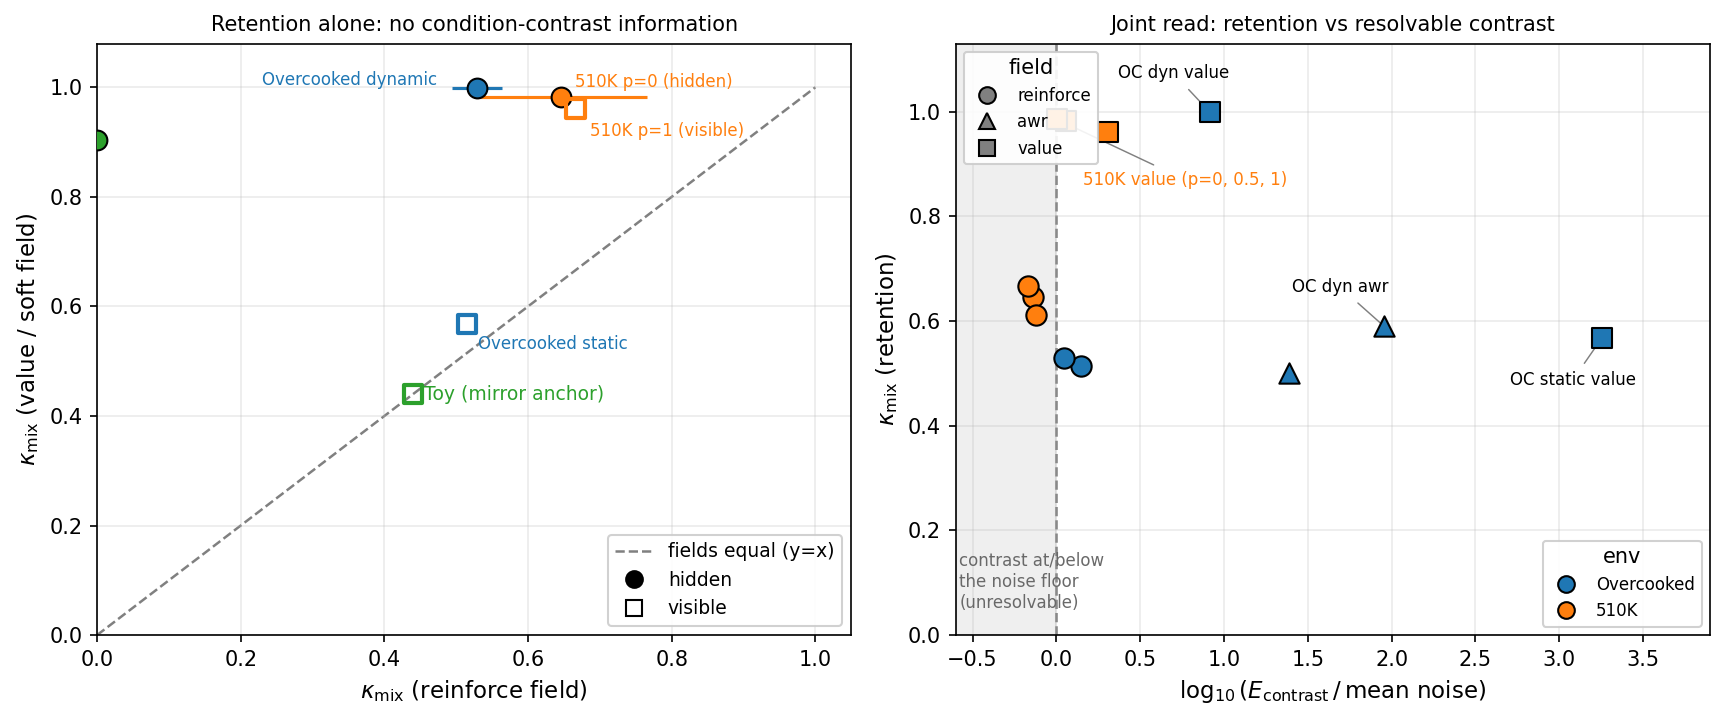
\includegraphics[width=0.85\linewidth]{../../figures/field_axis_comparison.png}
\end{center}
\caption{Retention alone and the joint diagnostic. Left: scatter under
$\kmix$ (condition means); retention separates the fields but carries no
information about their condition contrast. Right: $\kmix$ against the
condition contrast over the mean-estimation noise floor (log scale); the
shaded band is unresolvable. The Overcooked dynamic value point (retention
$0.998$) has a contrast share of $0.1\%$ and is condition-blind, as are the
510K value points; only the differentiable-baseline advantage fields sit
clearly above the floor with a substantial contrast share. The mirror-bandit
point is an exact anchor, not a real environment.}
\label{fig:field-axis}
\end{figure}

\subsection{Capacity, not optimizer}
\label{sec:exp-capacity}

On an exact $K$-way training comparison with a shared policy versus a
condition-aware policy (full-batch, deterministic, same initial logits), the
shared model's limitation is a mixture compromise
(Table~\ref{tab:capacity}). With a uniform mixture and the linear objective,
the shared model stays at average reward $0.667$ while the conditional model
reaches $1.99$ ($\kmix=0$ at initialization, by cancellation). Under mild and
strong asymmetric mixtures the shared model improves the average ($1.20$ and
$1.60$) but leaves the worst condition at $0.003$ and $0.002$, while the
conditional model keeps the worst condition at $1.97$ and $1.93$. The entropy channel ($\alpha=2$) trades average for worst-condition
performance ($0.752$/$0.517$), a Pareto movement rather than a fix. The intervention suggested by the audit is
conditional information or capacity, not an arbitrary gradient rule.

\begin{table}[t]
\caption{Shared versus condition-aware capacity (exact full-batch training).
Rewards are reported as average / worst condition.}
\label{tab:capacity}
\begin{center}
\begin{tabular}{llccc}
\toprule
Mixture & Model & avg.\ reward & worst reward & initial $\kmix$ \\
\midrule
uniform & shared, $\alpha{=}0$ & $0.667$ & $0.466$ & $0.000$ \\
uniform & conditional, $\alpha{=}0$ & $1.992$ & $1.992$ & — \\
mild & shared, $\alpha{=}0$ & $1.197$ & $0.003$ & $0.208$ \\
mild & conditional, $\alpha{=}0$ & $1.991$ & $1.970$ & — \\
mild & shared, $\alpha{=}2$ & $0.752$ & $0.517$ & $0.445$ \\
strong & shared, $\alpha{=}0$ & $1.597$ & $0.002$ & $0.501$ \\
strong & conditional, $\alpha{=}0$ & $1.991$ & $1.933$ & — \\
\bottomrule
\end{tabular}
\end{center}
\end{table}

\subsection{Real three-group preference data}
\label{sec:exp-dices}

To test whether the audit extends beyond RL bandits, we use DICES-350
\citep{arroyo2023dices}: 350 adversarial conversations, each rated by all 123
raters, with rater demographics; the dataset is released under CC BY 4.0. We
treat a demographic attribute as the hidden condition, use
the binary perceived-harm judgment (\texttt{Yes} vs \texttt{No},
\texttt{Unsure} dropped), split by \texttt{item\_id} (245 train / 105 test
items), and fit a TF-IDF plus logistic model shared across raters. Three
seeds; the shared model reaches $0.73$ train accuracy. Table~\ref{tab:dices}
reports the audit and the capacity comparison. The audit uses the BCE data
gradient (the condition-independent $L_2$ term shifts every condition mean
alike and cancels from $E_{\mathrm{contrast}}$/$\sigma^2$), with empirical
rater-frequency weights.

\begin{table}[t]
\caption{DICES-350 supervised check (three seeds). The race axis carries the
strongest condition signal, but its contrast energy is dominated by
within-group item noise, and conditional capacity yields no held-out gain.}
\label{tab:dices}
\begin{center}
\begin{tabular}{lcccc}
\toprule
Axis (groups) & $\kmix$ & $E_{\mathrm{contrast}}$ & $\sigma^2$ &
shared / cond.\ avg--worst \\
\midrule
race (3) & $0.156\pm0.027$ & $0.0019$ & $0.0114$ & $0.656/0.609$ / $0.654/0.607$ \\
age (3) & $0.002\pm0.000$ & $0.0002$ & $0.0058$ & $0.640/0.623$ / $0.638/0.624$ \\
gender (2) & $0.001\pm0.000$ & $0.0005$ & $0.0035$ & $0.641/0.623$ / $0.640/0.625$ \\
\bottomrule
\end{tabular}
\end{center}
\end{table}

On the race axis, the contrast energy is about six times smaller than the
within-group item noise ($E_{\mathrm{contrast}}/\sigma^2\approx0.17$), and
group-conditioned models do not improve average or worst-group accuracy. The
audit therefore predicts that this is not a capacity problem, and the
held-out comparison confirms it. This complements the bandit capacity
experiment: there, contrast dominates noise and condition-aware capacity
raises the worst condition from $0.003$ to $1.97$; here, contrast is
noise-dominated and conditional capacity buys nothing. Caveats:
\texttt{Q\_overall} is perceived harm, not objective harm; \texttt{Unsure} is
dropped; the model is a linear bag-of-ngrams classifier without group-DRO or
reweighting baselines.

\subsection{Retention is not a performance score}
\label{sec:exp-o4}

In a switching hidden-matching task with four objectives trained from scratch
under an identical budget (eight seeds), final returns and final structural
retention are shown in Table~\ref{tab:o4}. The arm with the lowest measured
retention is the best performer. The explanation is variable mismatch: the
task requires tracking a phase from reward history, which is orthogonal to the
initial partner label that retention conditions on. The diagnostic answers
``how much of the specified condition signal survives averaging,'' not ``will
training succeed.'' A low retention score must therefore be paired with a
check that the condition is the variable the task actually relies on. The
\texttt{awr} arm in this table uses a detached value baseline with advantages
clipped to $[-4,4]$; it is a different field from the differentiable-baseline
\texttt{awr} measured in Section~\ref{sec:exp-real} and in
Appendix~\ref{app:awr}. The \texttt{td} entry is a critic-loss gradient on the
arm's own $\epsilon$-greedy rollouts, a critic diagnostic rather than a
policy-gradient field; each arm is scored on its own rollouts.

\begin{table}[t]
\caption{Switching task: objectives trained from scratch under an identical
budget. Post-switch reward is measured on steps $20$--$28$ after the flip.}
\label{tab:o4}
\begin{center}
\begin{tabular}{lccc}
\toprule
Arm & return & post-switch reward & final $\kmix$ \\
\midrule
\texttt{td} & $\mathbf{36.97\pm0.06}$ & $0.75$ & $0.06\pm0.04$ \\
\texttt{softq} & $28.62\pm11.81$ & $0.58$ & $0.94\pm0.09$ \\
\texttt{reinforce} & $9.48\pm5.13$ & $0.18$ & $0.43\pm0.18$ \\
\texttt{awr} & $5.03\pm2.02$ & $0.04$ & $0.57\pm0.08$ \\
\bottomrule
\end{tabular}
\end{center}
\end{table}

\section{What the Audit Does and Does Not Claim}
\label{sec:claims}

The retained statements are: (i) exact cancellation conditions on the mirror
and matching models; (ii) an exact closed form for the soft-Q field and the
differentiable-baseline exception; (iii) $K$-way direction dependence and
channel interference as geometry; (iv) protocol and noise separation as
methodology; (v) a joint diagnostic in which a high retention with a
negligible contrast share is condition-blindness (the Overcooked dynamic
value field, and value in 510K), a contrast at the estimation-noise floor is
unresolvable (the plain policy gradient in Overcooked), and in 510K the
contrast stays at the noise floor or a few percent of the shared mass, and
only the differentiable-baseline advantage
field in Overcooked shows a resolvable, substantial contrast; and (vi)
decoupling from performance. The operational rule: condition-aware capacity is
the intervention when retention is low, contrast exceeds the estimation-noise
floor, and the condition is task-relevant; when the contrast is unresolvable
or negligible, or the condition is irrelevant, no intervention is
recommended. We do not claim that value methods are universally better, that
policy-gradient fields always vanish, that direction dependence is
group-specific, that retention predicts return, or that memory or entropy
interventions fix cancellation.

\section{Limitations}
\label{sec:limitations}

The exact results are bandit-level. Real-environment claims rest on
condition-mean gradients under one measurement protocol and on small seed
counts (three seeds for the Overcooked field axis). The value field is the
diagnostic $-\sum V$, not a TD residual; its score is dominated by the fitted
value function's condition-independent component on the measured
distribution, which the retention ratio does not penalize. Retention compares
condition means within one field; ranking $\kmix$ across objectives with
different supports in the padded parameter vector is not licensed. The Overcooked
\texttt{awr} entry uses the observed return-to-go as the advantage sample and
the learned value head as the differentiable baseline, so it is the practical
analogue of the analytic field; its per-step weights are computed in float64
under a dataset-level stop-gradient shift, a positive scalar multiple that
leaves $\kmix$ unchanged (float32 underflowed up to $78\%$ of the steps to
exactly zero, and the float64 re-run reproduces every score to within
$1.5\times10^{-7}$). The 510K environment has
weak relational drive and is used as a supporting measurement, not as the
primary demonstration. Its checkpoints were trained under a legacy action mask
that always enabled the pass bit; the mask-respecting evaluation corrects the
measurement side and does not require retraining. The real-data check uses a
single dataset (DICES-350), a linear TF-IDF model, and binary labels, without
conditional-routing, group-DRO, or reweighting baselines; a second dataset is
left to future work. The finite-sample analysis reports a
deterministic surrogate; a high-probability guarantee for the ratio estimator
would require an explicit distributional assumption.

\subsection*{Reproducibility statement}

The metric implementation is \texttt{src/iigc/metrics/kappa.py}; the closed
forms, protocol and visibility controls, $K$-way controls, Overcooked and 510K
measurements, and the capacity comparison are scripted under
\texttt{experiments/common\_basis/}. Result files carry a
\texttt{measurement\_metadata} block recording the gradient definition,
condition weights, rollout protocol, parameter space, and noise treatment.
Unit tests cover the closed forms, cancellation, boundedness, and the
metadata contract. No human subjects or private data are involved. Full
provenance is listed in Appendix~\ref{app:provenance}.

\subsection*{AI use statement}

In this work, we used generative AI tools for drafting assistance and code
editing suggestions. We have reviewed and verified all AI-assisted work: all
closed-form results were checked against independent autograd and Monte Carlo
computations, and all reported numbers are regenerated by the scripts listed
in Appendix~\ref{app:provenance}. We take responsibility for the final
content of this work.

\subsection*{Ethics statement}

This work studies optimization diagnostics for models trained on mixtures of
hidden subpopulations. It does not involve human subjects or private data. The
discussed failure mode (minority conditions being under-represented by
averaged objectives) has fairness implications; we present the audit as a
diagnostic and make no deployment recommendation.

\bibliography{references}
\bibliographystyle{iclr2027_conference}

\appendix

\section{Differentiable-baseline closed form}
\label{app:awr}

For the advantage-weighted field with $w=\exp((Q_r-V)/\tau)$ and a
differentiable baseline $V=\sum_a\pi(a)Q_r(a)$, write $x=2r/\tau$,
\begin{align}
A_0&=e^{xq}, & A_1&=e^{-xp}, & M_A&=p\log p\,A_0+q\log q\,A_1, \\
B_0&=e^{-xq}, & B_1&=e^{xp}, & M_B&=p\log p\,B_0+q\log q\,B_1,
\end{align}
with $p=\pi(\text{action }0)$, $q=1-p$. Then
\begin{equation}
c_A = pq\,(A_1-A_0+xM_A), \qquad
c_B = pq\,(B_1-B_0-xM_B).
\end{equation}
At $p=1/2$ the field cancels exactly for every $\tau$; otherwise retention
is monotone decreasing in $\tau$, with supremum $1/2$ as $\tau\to0$. Closed
form and autograd agree to
$9.2\times10^{-16}$ and Monte Carlo anchors agree within three standard
errors (\texttt{verify\_closed\_forms\_o1.py}).

\section{Number provenance}
\label{app:provenance}

\begin{table}[h]
\caption{Provenance of the main-text numbers.}
\label{tab:provenance}
\begin{center}
\small
\begin{tabular}{p{0.36\linewidth}p{0.58\linewidth}}
\toprule
Result & File or script \\
\midrule
Cancellation, soft-Q and AWR closed forms & \path{data/kappa/toy_fields/o1_closed_forms.json} \\
$K$-way cancellation, direction, interference & \path{data/kappa/toy_fields/kway_geometry.json} \\
Protocol audit (deterministic vs stochastic) & \path{data/kappa/toy_fields/det_vs_stoch.json} \\
Controlled visibility contrast (mirror bandit) & \path{data/kappa/toy_fields/visibility_control.json} \\
Overcooked field axis (shared episode batch) & \path{data/kappa/server_tasks/results/oc_field_axis.json} \\
Overcooked switch and memory protocol & \path{data/kappa/server_tasks/results/oc_switch_kappa.json} \\
510K paired protocol & \path{data/kappa/server_tasks/results/510k_field_axis.json} \\
Shared vs conditional capacity & \path{data/kappa/compromise_training/results.json} \\
Switching-task decoupling & \path{data/kappa/o4_adaptive/aggregate.json} \\
DICES-350 supervised check & \path{data/kappa/dices350/audit.json} \\
Canonical metric implementation & \path{src/iigc/metrics/kappa.py} \\
\bottomrule
\end{tabular}
\end{center}
\end{table}

\section{Correction log}
\label{app:corrections}

Superseded claims and their replacements are recorded in
\texttt{notes/paper1\_propositions\_corrections.md}, including the withdrawn
soft-Q dynamics claim, the parameter-space scope of the Fisher/KL variant, and
the replacement of $S_3$-specific language with $K$-way simplex geometry.

\end{document}
